

\section{User Interface}
\subsection{Authentifizierung}
Zur Authentifizierung der Benutzer wird der oAuth 2 Standard verwendet. Dieser erlaubt ein Login mit einem GitHub, FaceBook oder anderem Konto. Implementiert wurde dieser Standard auf der REST Seite mit Hilfe von verschiedenen Django Plugins. 
Beispielsweise wurde python-social-auth verwendet um den Benutzer gegenüber diesen Diensten zu authentisieren. Die REST Schnittstelle wird dann über einen Token gesichert.

\subsection{Transformationen erstellen}
Im Grundsatz wollten wir das Erstellen einer Transformation so einfach wie möglich gestalten. Zu diesem Zweck haben wir uns früh dazu entschlossen, einen Wizard zu schreiben, welcher die Aktion vereinfachen soll. In den frühen Phasen des Projektes war es notwendig den Wizard zu verwenden. In der Beta, die ausgeliefert wurde kann der Wizard verwendet werden, muss aber dank der Möglichkeit Tabellen ``zu laden'' nicht.
\begin{figure}[H]
\centering
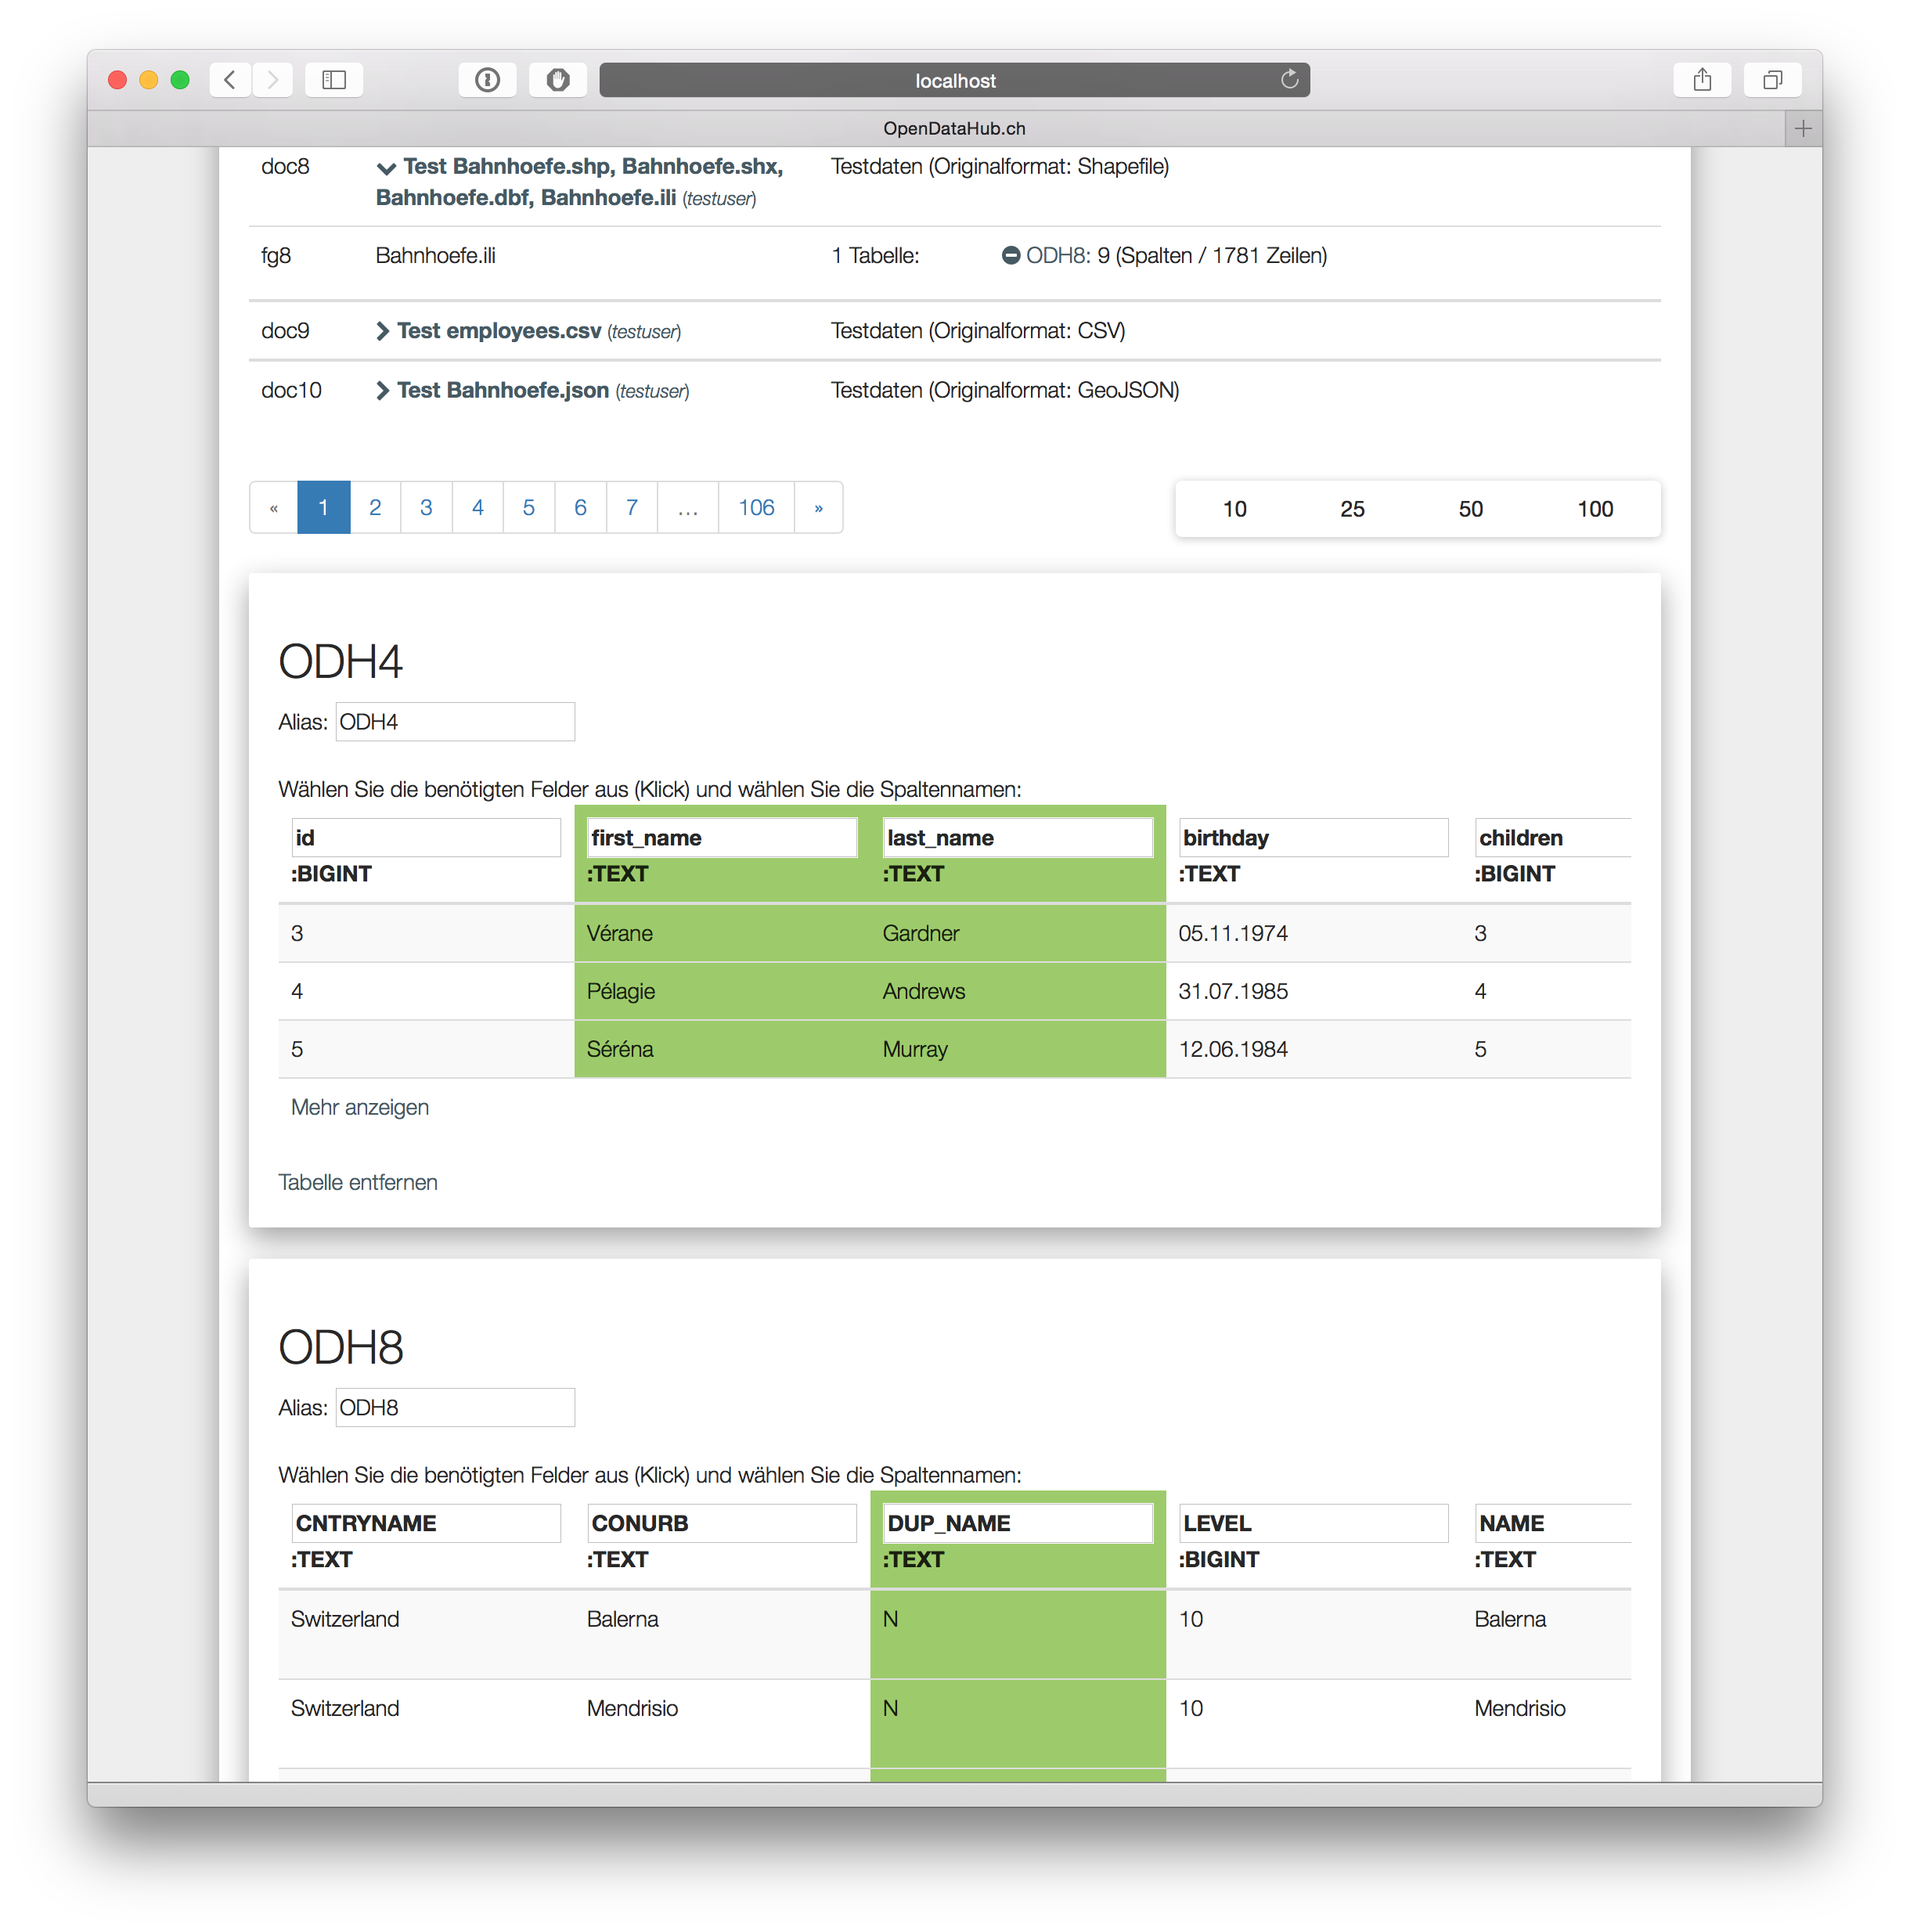
\includegraphics[width=\linewidth]{fig/odhql_wizard_early.png}
\caption{Tabellen können per Klick verbunden werden }
\label{fig:pd:tables_per_click}
\end{figure}
\begin{figure}[H]
\centering
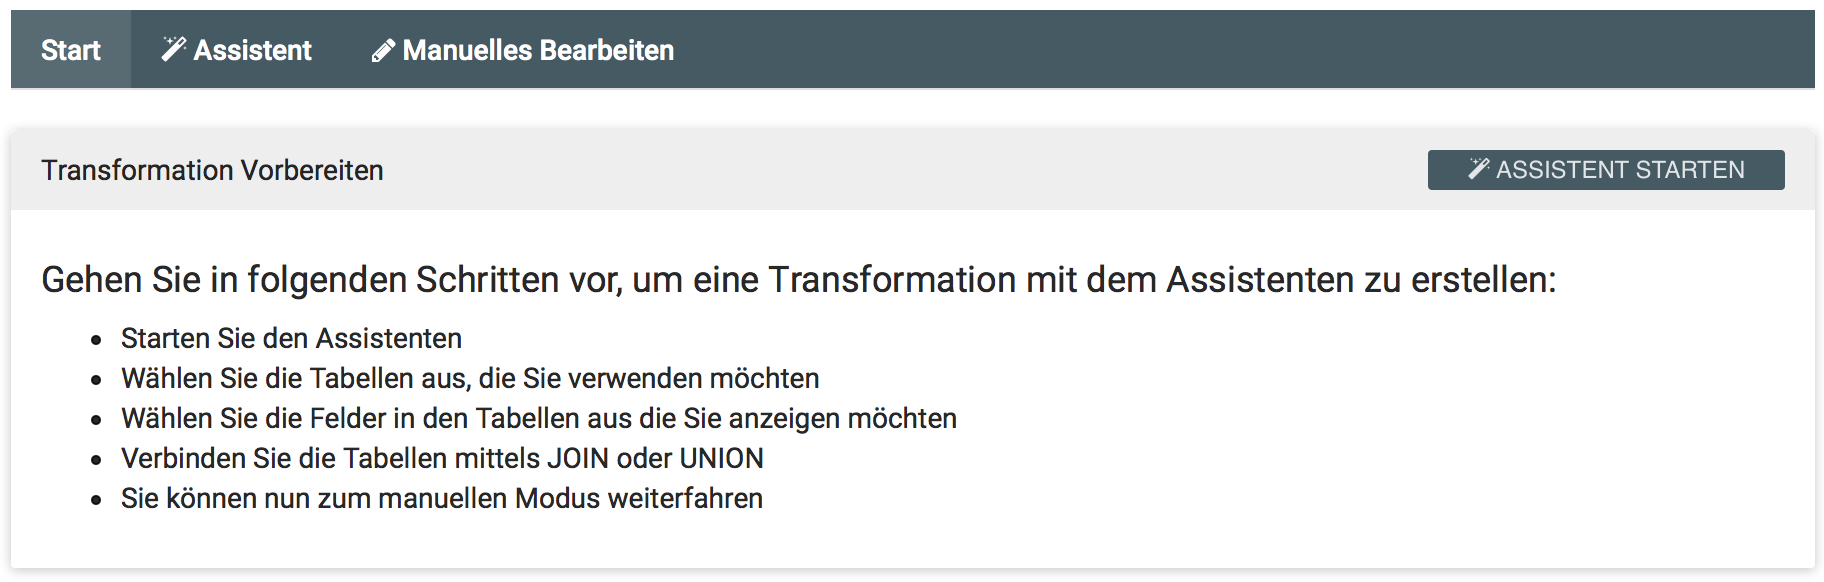
\includegraphics[width=\linewidth]{fig/wizard-step-one.png}
\caption{Einleitung in den Wizard}
\label{fig:pd:wizard-step-one}
\end{figure}
In einem ersten Schritt kann eine Transformation grundlegend erstellt werden. Einfache JOIN und UNION Operationen werden vom Benutzer konfiguriert.
\begin{figure}[H]
\centering
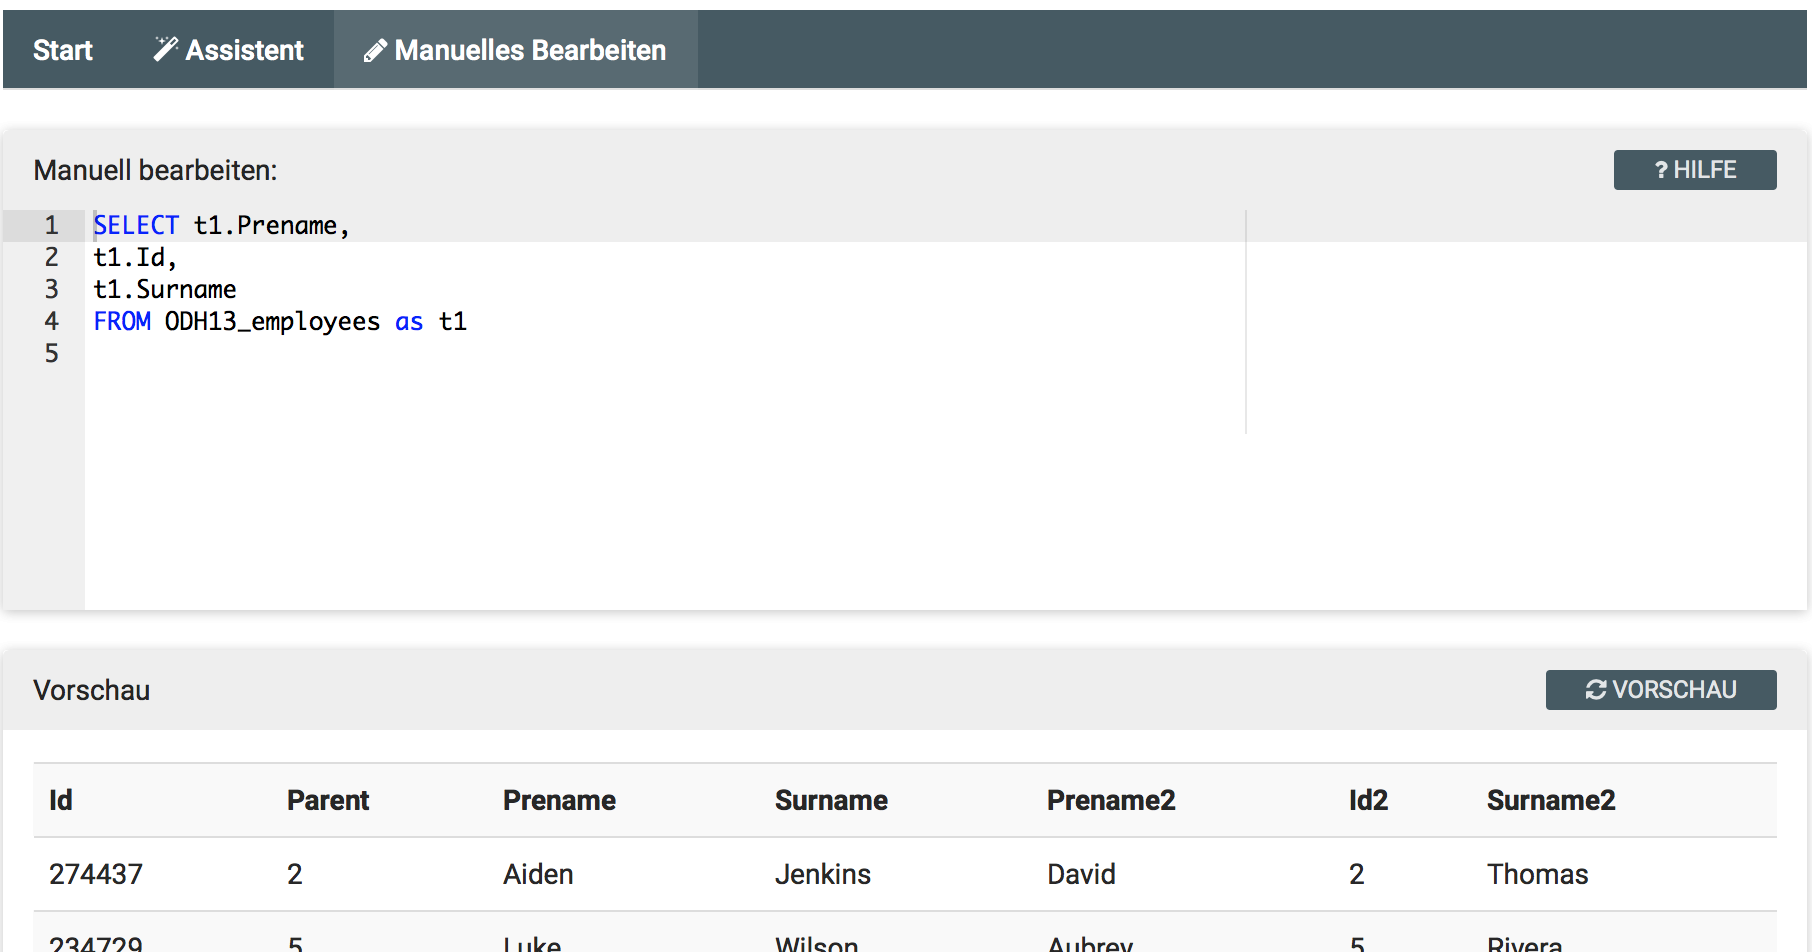
\includegraphics[width=\linewidth]{fig/wizard-manual.png}
\caption{Transformation manuell bearbeiten}
\label{fig:pd:wizard-manual}
\end{figure}

Später können dann die komplexeren Operationen auf die Daten angewendet werden. Hierfür wird der manuelle Modus verwendet. Im manuellen Modus steht eine Hilfe Seite zur Verfügung, welche sämtliche erweiterten Operationen erklärt.\\
Wird eine Transformation ``als Template'' verwendet, wird beim Speichern keine Prüfung der zugrunde legenden Daten durchgeführt. So können Syntaktisch korrekte, aber noch mit fehlenden Daten belastete Transformationen erstellt werden.

\subsection{Transformationen bearbeiten}
Transformationen können entweder geklont oder überschrieben werden. Beim Klonen legt der Benutzer eine neue Transformation auf Grund der Daten einer Bestehenden Transformation an. Beim Überschreiben kann der Besitzer einer Transformation diese verändern. Es kann bei diesen Operationen allerdings kein Wizard mehr verwendet werden, da dieser alle manuellen Änderungen überschreiben würde.
\begin{figure}[H]
\centering
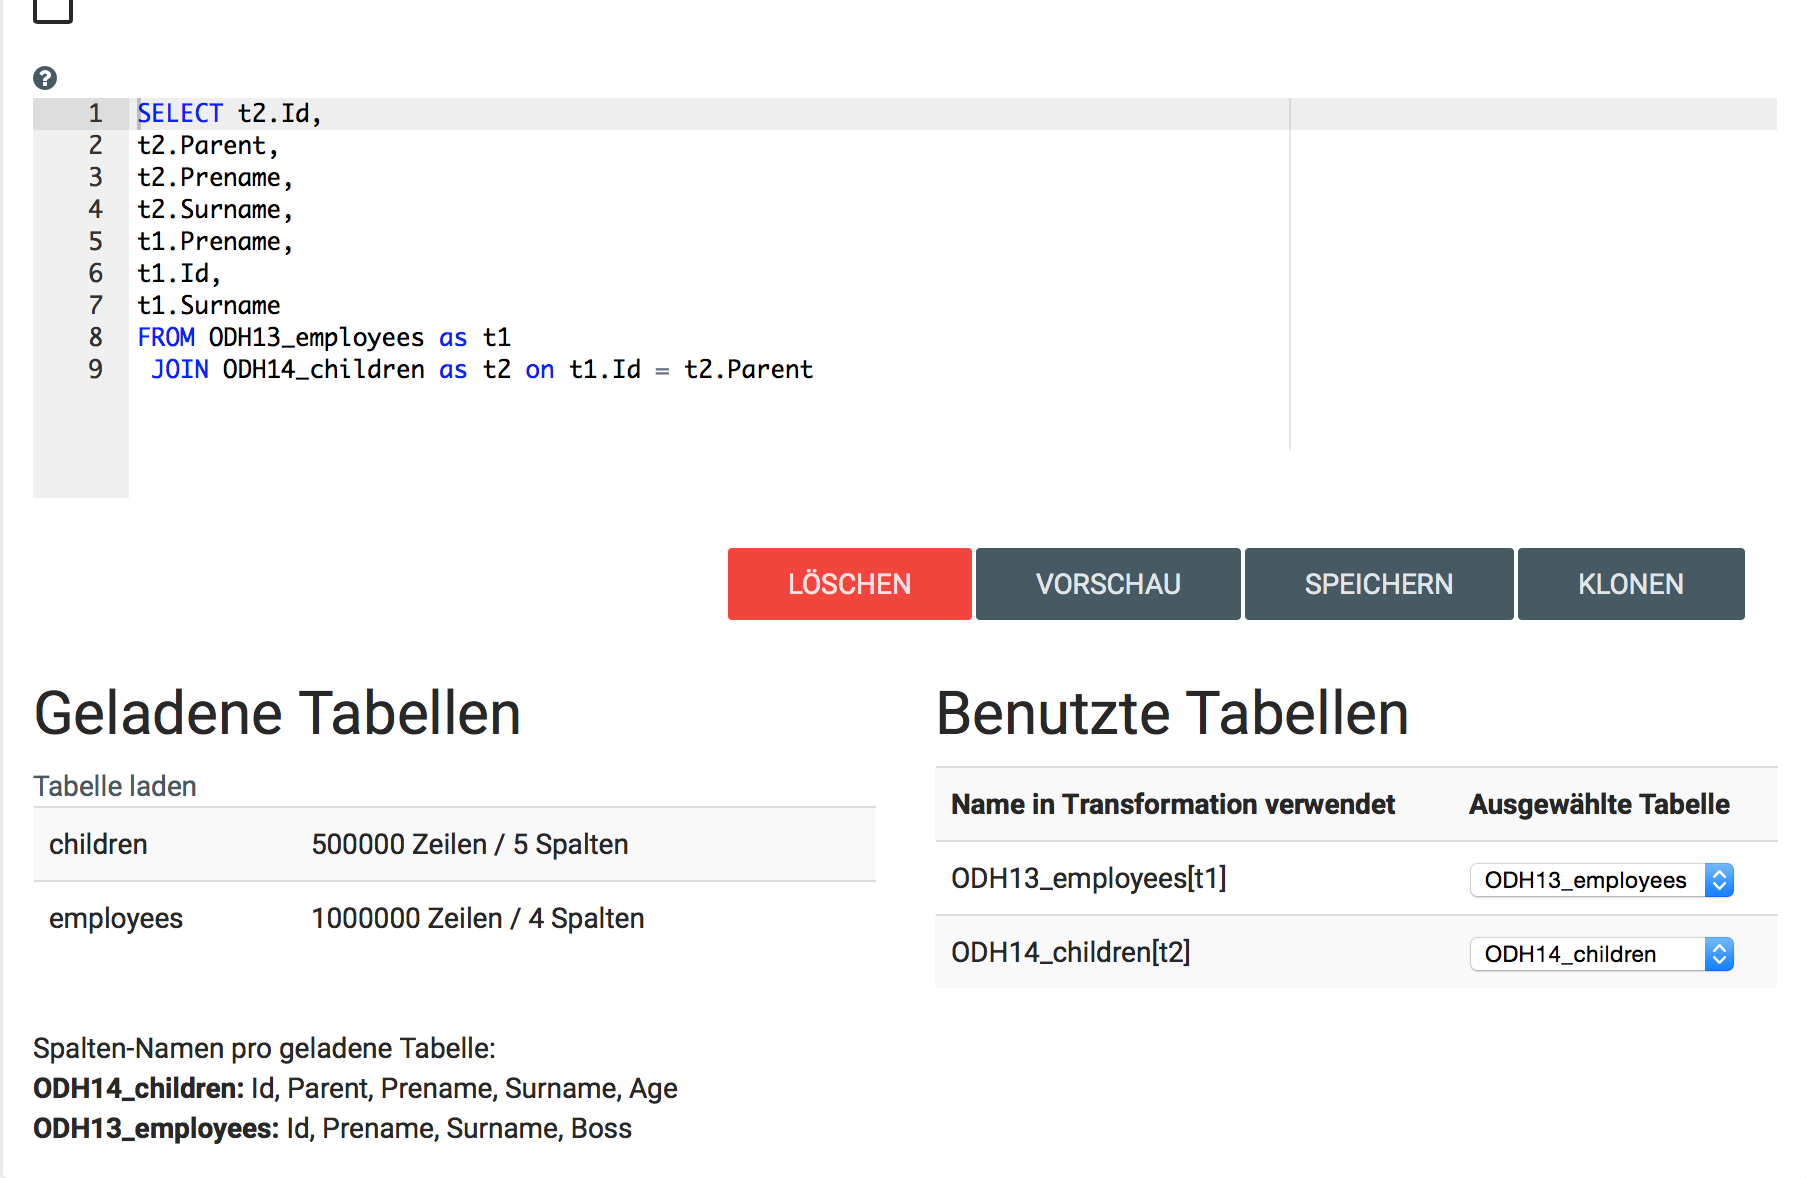
\includegraphics[width=\linewidth]{fig/transformation-edit.png}
\caption{Bestehende Transformation editieren}
\label{fig:pd:transformation-manual-edit}
\end{figure}